\section{Massively Learning Activities} \label{section: MLA}
TASI has been contracted by CNMI to create an infrastructure that allows for data analytics on Protected Health Information (PHI). This infrastructure will initially be hosted on-premises, with plans to move towards a hybrid solution in the future. To achieve this, we will be providing a Platform as a Service (PaaS) solution, by hosting SAS Viya services on our own hardware and allowing tenants to access and utilize the platform for their own analytics applications.

The tenants, including APCD, CMNI, CMA, Criminal Justice, and several Education environments, will provide the necessary data, which will be submitted to an ETL data pipeline for processing before being sent to SAS on-prem servers. Once the data has been processed, tenants may perform data analytics using advanced algorithms in SAS programming language.

To ensure secure operations, we will configure the security relationships between the software, hardware, and tenants using LDAP, security groups, encryption  and other related tools. Our goal is to architect a high-performance infrastructure that allows for advanced data analytics while maintaining the confidentiality and security of PHI.

Due to SAS being a time sensitive project, the initial deployment will have SAS suites and VMs installed on existing hardware, with plans to migrate the infrastructure to newly acquired hardware in the future.

\subsection{Planning}

The System Development Lifecycle (SDLC) is a project management model that defines different stages that are necessary to bring a project from conception to deployment and later maintenance. The SDLC model consists of several phases, which typically include requirements gathering, design, development, testing, deployment, and maintenance. The specific activities within each phase may vary depending on the project and the organization, but the basic principles are the same. The SDLC model is a flexible framework that can be adapted to suit the needs of different projects and organizations. It provides a systematic approach to software development that helps ensure that software is built efficiently, effectively, and with minimal risk.

Massively Learning Activities will follow a similar variation to the SDLC project management model where each SDLC stage will correspond to a subsection in this chapter. 

\subsection{Requirements of Analysis}
\textcolor{red}{Refer to the sizing documents (2) and the current resources document comparison to see what we are missing.}

\subsection{Security and Risks}
\textbf{Security In-Depth}
\begin{itemize}
    \item LDAP
    \item VMware Security Policies
    \item SAS Security Policies
    \item HIPPA, other Federal Laws
\end{itemize}

\subsection{Design and Protoyping I}
Massively Learning Activities (MLA) is divided into two phases, (1) the initial deployment of SAS on existing infrastructure and later (2) the migration of SAS onto scaled infrastructure. 

In either deployment stage, SAS Viya will be deployed in a multi-tenant environment. A multi-tenant deployment of SAS Viya allows for a single deployment to serve multiple customers\footnote{Customers are tenants (etc: CNMI, APCD, CMA, Med-Quest, UH Education) but each tenant has its own set of users and groups.}. These customers can share some physical resources while remaining logically separated. A multi-tenant deployment allows for these distinct groups to share IT resources in a secure and cost-effect manner. Multi-tenancy deploys into a \href{https://kubernetes.io/}{Kubernetes} namespace. The deployment includes a provider tenant, shared mid-tier services, application-specific database schemas, shared applications, and a designated SAS administrator for the provider tenant. Administrators with elevated Kubernetes privileges onboard one or more tenants. After tenant on-boarding, Kubernetes administrators onboard one or more Cloud Analytic Services into each new tenant, then each CAS server is uniquely configured during the on-boarding process to meet the specific tenant requirements. 

The final and completed deployment of SAS Viya will expect a total of 8 tenants:

\begin{itemize}
    \item \textbf{Tenant 1}: Commonwealth of the Northern Mariana Islands (CNMI)
    \item \textbf{Tenant 2}: All-Payer Claims Database (APCD)
    \item \textbf{Tenant 3}: Centers for Medicare \& Medicaid Services (CMA)
    \item \textbf{Tenant 4}: Med-Quest
    \item \textbf{Tenant 5}: UH Education 1
    \item \textbf{Tenant 6}: UH Education 2
    \item \textbf{Tenant 7}: UH Education 3
    \item \textbf{Tenant 8}: UH Education 4
\end{itemize}

\subsubsection{Initial Deployment}
\textbf{HARDWARE AND SOFTWARE}

The initial deployment of MLA will involve installing SAS Viya and SAS DMA on existing infrastructure\footnote{Infrastructure is used to describe existing hardware available to use on-premises at TASI/PHIDC.}. The existing infrastructure is  an available Dell PowerEdge FX2 Enclosure located in TASI's NOC. The PowerEdge FX2 Enclosure is a 2U hybrid rack-based computing platform that combines multiple blades\footnote{Blades are complete servers in a smaller form factor that have their own CPU(s), memory, storage, and networking components.} into a single enclosure to increase the efficiency and reduce the cost of rack-based systems. This multi-blade enclosure has a \textcolor{red}{XXGB} connection to a \textcolor{red}{storage pool (describe me)}.

Each blade is installed with \textbf{ESXi 6.7} as the host operating system and is equipped with \textbf{12 CPU(s) w/ XX cores}, \textbf{256GB} of RAM, and \textcolor{red}{\textbf{XXGB}} of personal storage. Theses resources will be logically separated to configure a multi-tenant environment. These virtual machines (VMs) will be created and managed through vCenter (and later through SAS), which is running on a separate server. The VMs responsible for a CAS role will use RHEL \textcolor{red}{7.X} as the host operating system. 

CNMI, APCD, CMA, and Med-Quest will be the initial four tenants with each tenant having their own  deployment configuration based on their respective requirements. CNMI and APDC will be configured in a 5-server environment \footnote{5 Server: (1) Primary CAS Controller, (2) Backup CAS Controller, (3) CAS Worker 1, (4) CAS Worker 2, (5) CAS Worker 3} and every other tenant will be configured in a 3-server environment\footnote{3 Server: (1) Primary CAS Controller, (2) Backup CAS Controller, (3) CAS Worker 1}. The other tenants that are yet to be added will be considered during the migration stage of MLA. 

\begin{figure}[H]
    \centering
    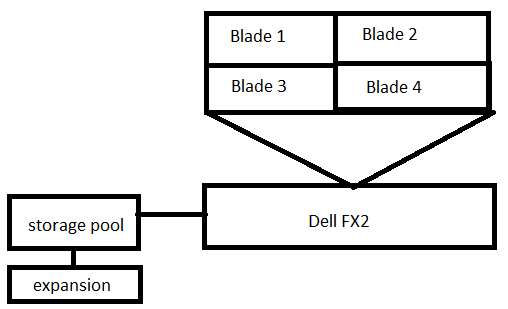
\includegraphics[scale = 0.75]{images/currentENV.png}
    \caption{TASI On-Premise Environment \textcolor{red}{(needs VISIO)} }
    \label{Current ENV}
\end{figure}

There are several factors that impact the configuration of SAS technologies in a virtualized environment:  \textbf{(1) high availability and redundancy}; \textbf{(2) optimization}; and \textbf{(3) security and compliance}. 

(1) Consider that although virtualizing the CAS Controller and Backup Controller on the same hardware can offer several benefits, such as cost savings, simplified management, and easier backup and recovery processes, it will be better to virtualize them on separate hardware to provide high availability and redundancy of CAS controllers (Figure 6.2), in the case of unexpected downtime. As for CAS Workers, it is recommended to virtualize them on separate hardware to reduce resource conflicts but it is not necessary. 

(2) The performance overhead of using SAS Viya and CAS on VMs instead of dedicated hardware can depend on several factors including workload characteristics, available hardware resources, and the virtualization technology used.

\textcolor{red}{In section 6.3.1, if the advantage of distributing the SAS components
across blades is for load balancing, it would be good to include a
comment to that effect -- otherwise, it would probably be more efficient
to have them all on the same blade.}

(3) In a logically separated multi-tenant environment, MLA must ensure network and data isolation between each tenant, data encryption for data at rest and in transit, a well configured access control list for hardware and software, and compliance certification for handling PHI data (i.e., HIPAA, PCI DSS, SOC 2, HITECH, Hawaii Information Privacy Act, etc). 

\begin{figure}[H]
    \centering
    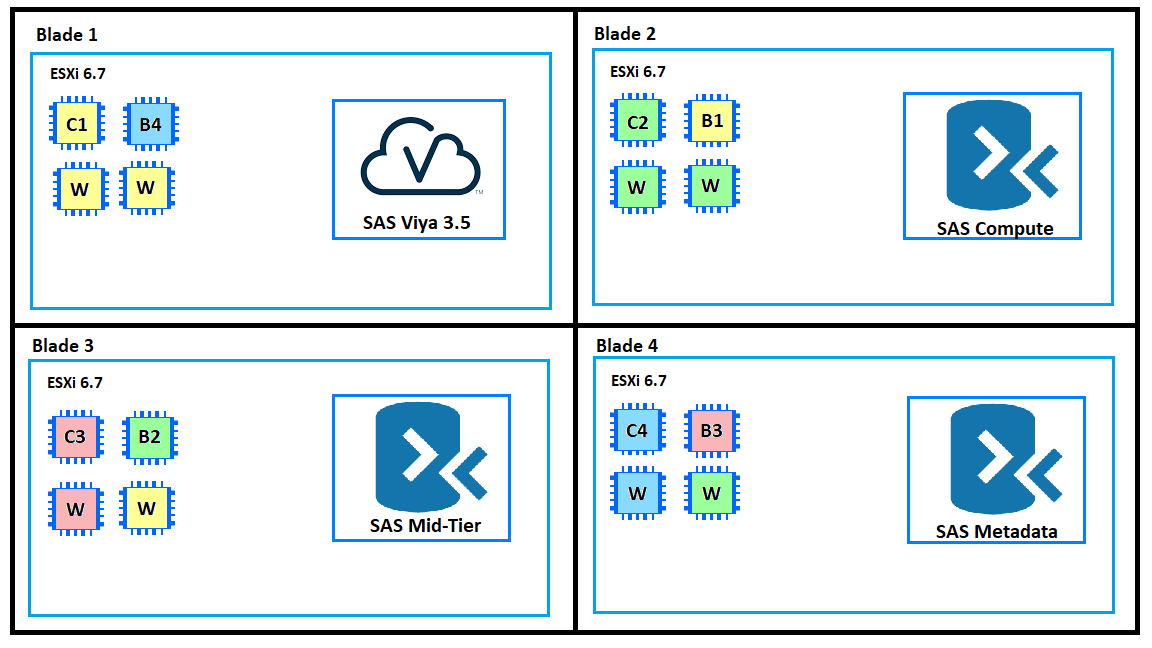
\includegraphics[scale = 0.52]{images/initial-deployment-diagram.png}
    \caption{Initial Multi-Tenant Deployment \textcolor{red}{(needs VISIO)} }
    \label{Initial Multi-Tenant Deployment}
\end{figure} 

To maximize resource efficiency, CAS nodes will be evenly distributed across each blade, where a blade will consist of one controller, one backup controller, and two workers. The controller and backup controller, configured on the same system, will belong to separate tenants. The workers will also belong to separate tenants but each blade will have at least one related controller and worker per system. 

Subsequently, four additional VMs will be created to support the installation of SAS Viya and SAS DMA. SAS Viya will be installed as software on top of a RHEL 3.7X VM instance, in Blade 1. SAS DMA consists of three software components that will installed as software on top of Windows Server 2019 VM instances, in Blades' 2, 3, and 4. 

\textbf{Security In-Depth}
\begin{itemize}
    \item LDAP
    \item VMware Security Policies
    \item SAS Security Policies
    \item HIPPA, other Federal Laws
\end{itemize}

\subsubsection{Migration Deployment}
The migration deployment of MLA will involve the migratin ghte vm's we ssetup in the intial deployment using vmware software suite VMotion. Vmotion!.

\subsection{Deployment and Prototyping I (Initial)}

\subsection{Testing \& Integration I}

\subsection{Operations and Maintenance I}

\subsection{Deployment and Prototyping II (Migration)}
\textcolor{red}{VMotion in action (See 6.1.2).}

\subsection{Testing \& Integration II}

\subsection{Operations and Maintenance II}

